\documentclass[12pt]{article}
\usepackage[fleqn]{amsmath}
\usepackage{amssymb}
\usepackage{amsthm}
\usepackage{amssymb}
\usepackage{tikz}
\usepackage{pgfplots}
    \pgfplotsset{width=10cm,compat=1.9}
\usepackage{tipa}
\usepackage{hyperref}
\usepackage{mathtools}
    \hypersetup{colorlinks=true,citecolor=blue,urlcolor =black,linkbordercolor={1 0 0}}
\newcommand*\circled[1]{\tikz[baseline=(char.base)]{
    \node[shape=circle,draw,inner sep=2pt] (char) {#1};}}
\newcommand{\BR}{\mathbb R}
\newcommand{\BN}{\mathbb N}
\newcommand{\prm}{^\prime}
\newcommand{\doubleprime}{^{\prime\prime}}
\newcommand{\phii}{\varphi}
\title{Lecture 22}
\begin{document}
\maketitle
\vspace*{-0.25in}
\begin{center}
	Anders Sundheim \\
	\href{mailto:asundheim@wisc.edu}{{\tt asundheim@wisc.edu}}
\end{center}
\subsection*{Change of Variables}
    \[ \iint_Sf(x,y)\,dx\,dy=\iint_Tf(r\cos(\theta),r\sin(\theta))r\,dr\,d\theta \]
\subsection*{Ex. 1}
    \[
        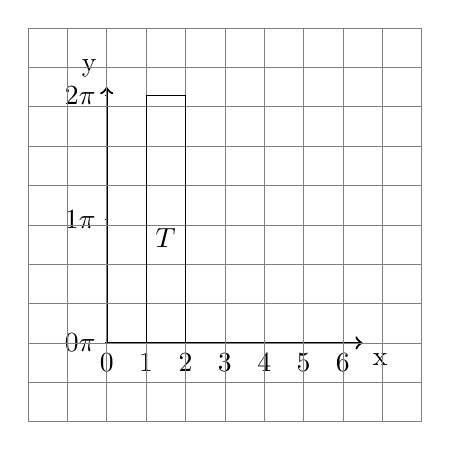
\begin{tikzpicture}[scale=0.5]
            \draw[thick,->] (0,0) -- (6.5,0) node[anchor=north west] {x};
            \draw[thick,->] (0,0) -- (0,6.5) node[anchor=south east] {y};
            \foreach \x in {0,1,2,3,4,5,6}
                \draw (\x cm,1pt) -- (\x cm,-1pt) node[anchor=north] {$\x$};
            \foreach \y in {0,1,2}
                \draw (1pt,3.14*\y cm) -- (-1pt,3.14*\y cm) node[anchor=east] {$\y\pi$};
            \draw[step=1cm,gray,very thin] (-2,-2) grid (8,8);
            \draw (1,0) rectangle (2, 2*pi);
            \draw (1.5,pi) node[anchor=north]{$T$};
        \end{tikzpicture}
        \xrightarrow[y=r\sin\theta]{x=r\cos\theta}
        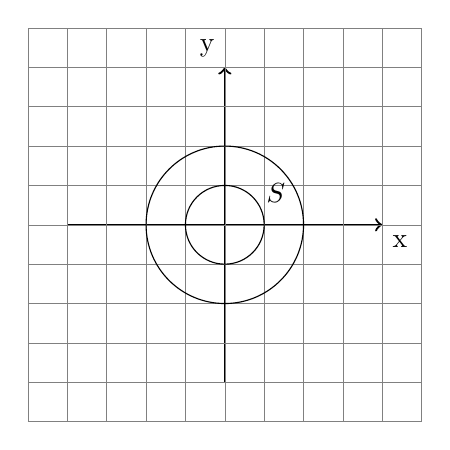
\begin{tikzpicture}[scale=0.5]
            \draw[thick,->] (-1,3) -- (7,3) node[anchor=north west] {x};
            \draw[thick,->] (3,-1) -- (3,7) node[anchor=south east] {y};
            \draw[step=1cm,gray,very thin] (-2,-2) grid (8,8);
            \draw (3, 3) circle (1);
            \draw (3, 3) circle (2);
            \draw (4.3,4.3) node[anchor=north]{$S$};
        \end{tikzpicture}
    \]
\subsection*{Ex. 2}
    \[ \iint_S\sqrt{1-x^2-y^2}\,dx\,dy \]
    \[ 
        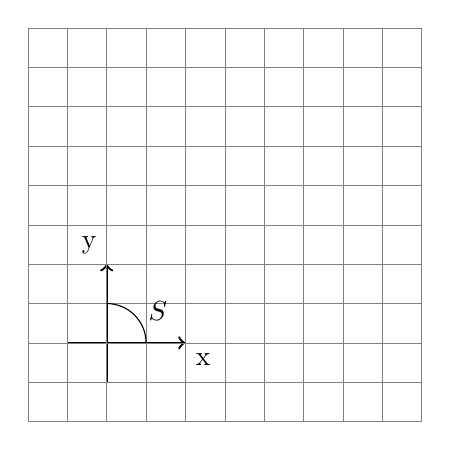
\begin{tikzpicture}[scale=0.5]
            \draw[thick,->] (-1,0) -- (2,0) node[anchor=north west] {x};
            \draw[thick,->] (0,-1) -- (0,2) node[anchor=south east] {y};
            \draw[step=1cm,gray,very thin] (-2,-2) grid (8,8);
            \draw (1, 0) arc (0:90:1);
            \draw (1.3,1.3) node[anchor=north]{$S$};
        \end{tikzpicture}
    \]
    \underline{Sln.} Use change of variables using polar coordinates \\
    \[
        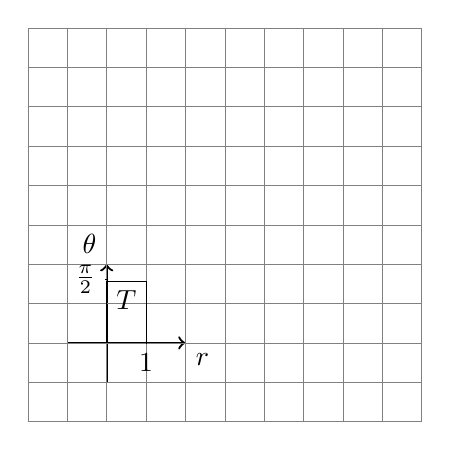
\begin{tikzpicture}[scale=0.5]
            \draw[thick,->] (-1,0) -- (2,0) node[anchor=north west] {$r$};
            \draw[thick,->] (0,-1) -- (0,2) node[anchor=south east] {$\theta$};
            \draw[step=1cm,gray,very thin] (-2,-2) grid (8,8);
            \draw (0, 0) rectangle (1, pi/2);
            \draw (.5,pi/2) node[anchor=north]{$T$};
            \draw (1pt,1.62 cm) -- (-1pt,1.62 cm) node[anchor=east] {$\frac{\pi}{2}$};
            \draw (1 cm,1pt) -- (1 cm,-1pt) node[anchor=north] {$1$};
        \end{tikzpicture}
    \]
    \[ T=[0,1]\times[0,\frac{\pi}{2}] \]
    \[ \iint_S\sqrt{1-x^2-y^2}\,dx\,dy=\iint_T\sqrt{1-r^2\cos^2\theta-r^2\sin^2\theta}r\,dr\,d\theta=\iint_T\sqrt{1-r^2}r\,dr\,d\theta \]
    \[ = \bigg(\int_0^{\frac{\pi}{2}}\,d\theta\bigg)\bigg(\int_0^1\sqrt{1-r^2}r\,dr\bigg) \]
    \[ 
        = \frac{\pi}{2}\int_0^1\frac{1-r^2}r\,dr\quad\quad 
        \begin{cases}
            u=1-r^2 \\
            du=-2r\,dr
        \end{cases}
    \]
    \[ =\frac{-\pi}{4}\int_1^0\sqrt{u}\,du=\frac{\pi}{4}\int_0^1\sqrt{u}\,du=\frac{\pi}{4}\frac{2}{3}u^{\frac{3}{2}}\bigg]_0^1=\frac{2\pi}{12}=\frac{\pi}{6} \]
\subsection*{Linear Transformations in Two Dimensions}
    \[
        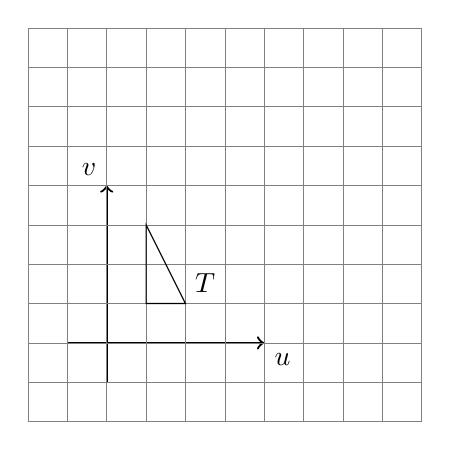
\begin{tikzpicture}[scale=0.5]
            \draw[thick,->] (-1,0) -- (4,0) node[anchor=north west] {$u$};
            \draw[thick,->] (0,-1) -- (0,4) node[anchor=south east] {$v$};
            \draw[step=1cm,gray,very thin] (-2,-2) grid (8,8);
            \draw (1, 1) -- (2,1) -- (1,3) -- cycle;
            \draw (2.5,2) node[anchor=north]{$T$};
        \end{tikzpicture}
        \xrightarrow[x=Au+Bv]{y=Cu+Dv}
        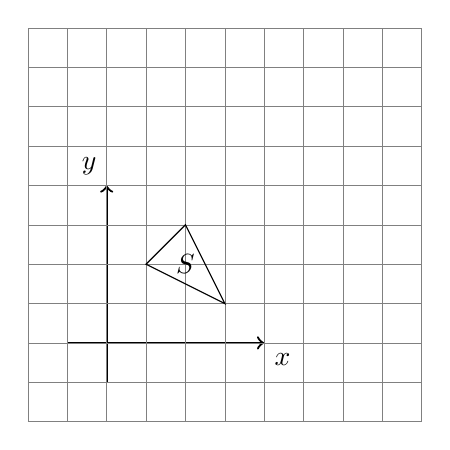
\begin{tikzpicture}[scale=0.5]
            \draw[thick,->] (-1,0) -- (4,0) node[anchor=north west] {$x$};
            \draw[thick,->] (0,-1) -- (0,4) node[anchor=south east] {$y$};
            \draw[step=1cm,gray,very thin] (-2,-2) grid (8,8);
            \draw (1, 2) -- (3,1) -- (2,3) -- cycle;
            \draw (2,2.5) node[anchor=north]{$S$};
        \end{tikzpicture}
    \]
    Q: $\iint_Sf(x,y)\,dx\,dy$ \\
    S: a polygon in 2D \\
    We need to find what is $J(u,v)$? \\
    \[
        J(u,v)=
        \begin{vmatrix}
            A & B \\
            C & D
        \end{vmatrix}    
        =
        \begin{vmatrix}
            \frac{dx}{du} & \frac{dy}{du} \\
            \frac{dx}{dv} & \frac{dy}{dv}
        \end{vmatrix}
        =
        \begin{vmatrix}
            A & C \\
            B & D
        \end{vmatrix}
        = AD-BC
    \]
    \underline{Condition we need} $AD-BC\neq 0\rightarrow$ the linear map \\
    $(u,v)\mapsto (x,y)$ is 1-to-1 \\
    Change of variables formula: \\
    \[ \iint_Sf(x,y)\,dx\,dy=\iint_Tf(Au+Bv,Cu+Dv)|AD-BC|\,du\,dv \]
    \[ |AD-BC|\iint_Tf(Au+Bv,Cu+Dv)\,du\,dv \]
\subsection*{Ex. 1}
    Let $f=1$, then we have: \\
    Area of $S=|AD-BC|\cdot$(Area of $T$) \\
    \[
        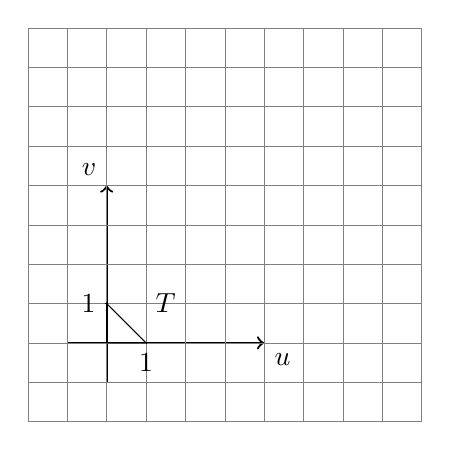
\begin{tikzpicture}[scale=0.5]
            \draw[thick,->] (-1,0) -- (4,0) node[anchor=north west] {$u$};
            \draw[thick,->] (0,-1) -- (0,4) node[anchor=south east] {$v$};
            \draw[step=1cm,gray,very thin] (-2,-2) grid (8,8);
            \draw (0, 0) -- (0,1) -- (1,0) -- cycle;
            \draw (1.5,1.5) node[anchor=north]{$T$};
            \draw (1pt,1 cm) -- (-1pt,1 cm) node[anchor=east] {$1$};
            \draw (1 cm,1pt) -- (1 cm,-1pt) node[anchor=north] {$1$};
        \end{tikzpicture}
        \xrightarrow[y=3v]{x=\frac{1}{3}u}
        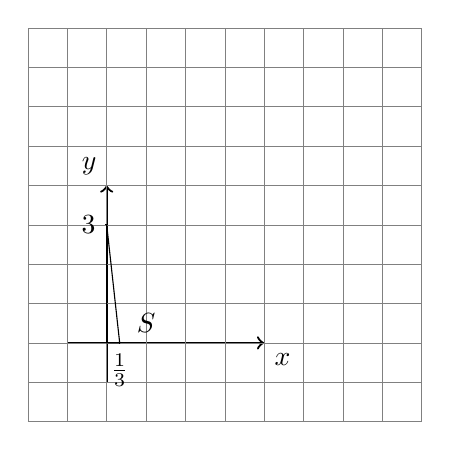
\begin{tikzpicture}[scale=0.5]
            \draw[thick,->] (-1,0) -- (4,0) node[anchor=north west] {$x$};
            \draw[thick,->] (0,-1) -- (0,4) node[anchor=south east] {$y$};
            \draw[step=1cm,gray,very thin] (-2,-2) grid (8,8);
            \draw (0, 0) -- (.33,0) -- (0,3) -- cycle;
            \draw (1,1) node[anchor=north]{$S$};
            \draw (1pt,3 cm) -- (-1pt,3 cm) node[anchor=east] {$3$};
            \draw (.33 cm,1pt) -- (.33 cm,-1pt) node[anchor=north] {$\frac{1}{3}$};
        \end{tikzpicture}
    \]
    \[
        \begin{vmatrix*}
            A & C \\
            B & D
        \end{vmatrix*}     
        =
        \begin{vmatrix*}
            \frac{1}{3} & 0 \\
            0 & 3
        \end{vmatrix*}
        = 1
    \]
\subsection*{Ex. 2}
    \[
        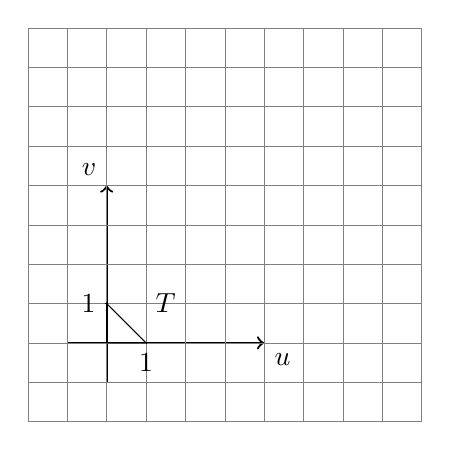
\begin{tikzpicture}[scale=0.5]
            \draw[thick,->] (-1,0) -- (4,0) node[anchor=north west] {$u$};
            \draw[thick,->] (0,-1) -- (0,4) node[anchor=south east] {$v$};
            \draw[step=1cm,gray,very thin] (-2,-2) grid (8,8);
            \draw (0, 0) -- (0,1) -- (1,0) -- cycle;
            \draw (1.5,1.5) node[anchor=north]{$T$};
            \draw (1pt,1 cm) -- (-1pt,1 cm) node[anchor=east] {$1$};
            \draw (1 cm,1pt) -- (1 cm,-1pt) node[anchor=north] {$1$};
        \end{tikzpicture}
        \xrightarrow[y=(-u+v)\sqrt{2}]{x=\frac{u+v}{\sqrt{2}}}
        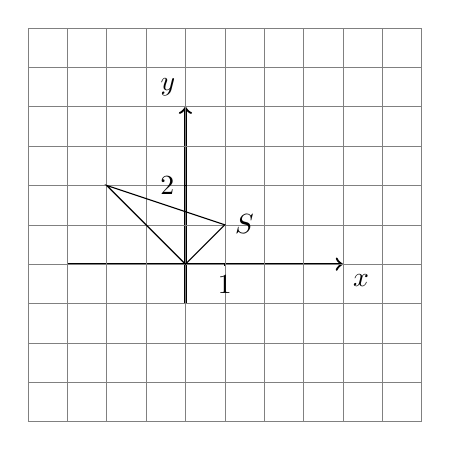
\begin{tikzpicture}[scale=0.5]
            \draw[thick,->] (-3,0) -- (4,0) node[anchor=north west] {$x$};
            \draw[thick,->] (0,-1) -- (0,4) node[anchor=south east] {$y$};
            \draw[step=1cm,gray,very thin] (-4,-4) grid (6,6);
            \draw (0, 0) -- (1,1) -- (-2,2) -- cycle;
            \draw (1.5,1.5) node[anchor=north]{$S$};
            \draw (1pt,2 cm) -- (-1pt,2 cm) node[anchor=east] {$2$};
            \draw (1 cm,1pt) -- (1 cm,-1pt) node[anchor=north] {$1$};
        \end{tikzpicture}
    \]
    \[ 
        \begin{vmatrix*}
            A & C \\
            B & D
        \end{vmatrix*}
        =
        \begin{vmatrix*}
            \frac{1}{\sqrt{2}} & -\sqrt{2} \\
            \frac{1}{\sqrt{2}} & \sqrt{2}
        \end{vmatrix*}
        = 2
    \]
    \[ |AD-BC| = \frac{\text{Area of $S$}}{\text{Area of $T$}} \]
\subsection*{Ex. 3}
    \[
        \iint_Se^{\frac{y-x}{y+x}}\,dx\,dy     
    \]
    \[
        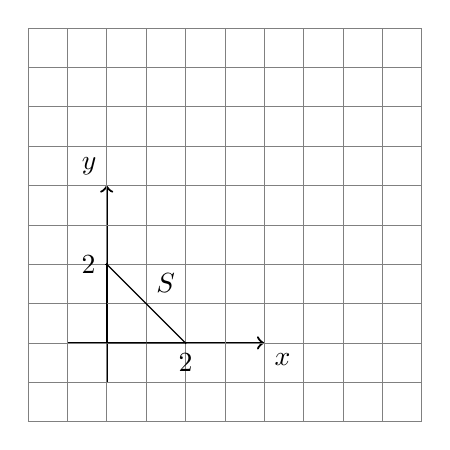
\begin{tikzpicture}[scale=0.5]
            \draw[thick,->] (-1,0) -- (4,0) node[anchor=north west] {$x$};
            \draw[thick,->] (0,-1) -- (0,4) node[anchor=south east] {$y$};
            \draw[step=1cm,gray,very thin] (-2,-2) grid (8,8);
            \draw (0, 0) -- (0,2) -- (2,0) -- cycle;
            \draw (1.5,2) node[anchor=north]{$S$};
            \draw (1pt,2 cm) -- (-1pt,2 cm) node[anchor=east] {$2$};
            \draw (2 cm,1pt) -- (2 cm,-1pt) node[anchor=north] {$2$};
        \end{tikzpicture}
    \]
    \[
        \begin{cases}
            u=y-x \\
            u=y+x
        \end{cases}
        \begin{vmatrix*}
            A & C \\
            B & D
        \end{vmatrix*}
        =
        \begin{vmatrix*}
            -\frac{1}{2} & \frac{1}{2} \\
            \frac{1}{2} & \frac{1}{2}
        \end{vmatrix*}
        = -\frac{1}{2}
    \]
    \[
        \Rightarrow
        \begin{cases}
            x=\frac{v-u}{2} \\
            y=\frac{u+v}{2}
        \end{cases}
    \]
    \[ \iint_Se^{\frac{y-x}{y+x}}\,dx\,dy=\iint_Te^{\frac{u}{v}}\frac{1}{2}\,du\,dv \]
    \[
        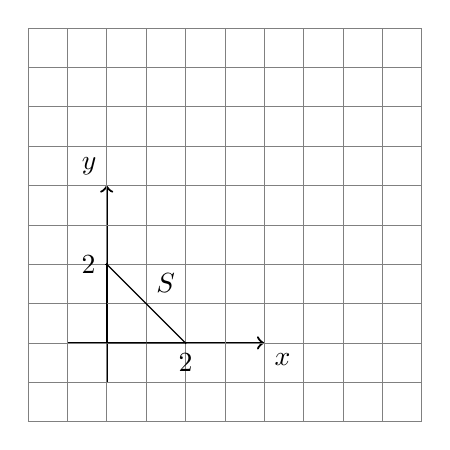
\begin{tikzpicture}[scale=0.5]
            \draw[thick,->] (-1,0) -- (4,0) node[anchor=north west] {$x$};
            \draw[thick,->] (0,-1) -- (0,4) node[anchor=south east] {$y$};
            \draw[step=1cm,gray,very thin] (-2,-2) grid (8,8);
            \draw (0, 0) -- (0,2) -- (2,0) -- cycle;
            \draw (1.5,2) node[anchor=north]{$S$};
            \draw (1pt,2 cm) -- (-1pt,2 cm) node[anchor=east] {$2$};
            \draw (2 cm,1pt) -- (2 cm,-1pt) node[anchor=north] {$2$};
        \end{tikzpicture}
        \quad\quad
        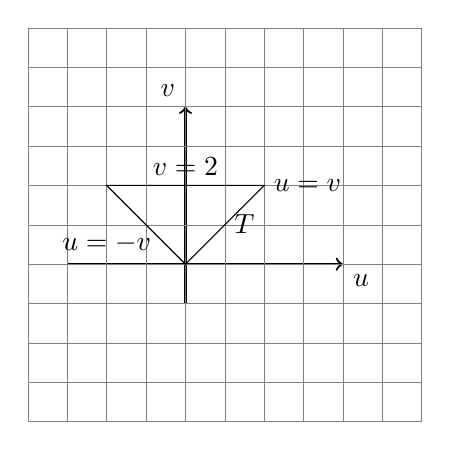
\begin{tikzpicture}[scale=0.5]
            \draw[thick,->] (-3,0) -- (4,0) node[anchor=north west] {$u$};
            \draw[thick,->] (0,-1) -- (0,4) node[anchor=south east] {$v$};
            \draw[step=1cm,gray,very thin] (-4,-4) grid (6,6);
            \draw (0, 0) -- (-2,2) -- (2,2) node[anchor=west]{$u=v$} -- cycle;
            \draw (0, 2) node[anchor=south]{$v=2$};
            \draw (-2, 1) node[anchor=north]{$u=-v$};
            \draw (1.5,1.5) node[anchor=north]{$T$};
        \end{tikzpicture}
    \]
    \[
       =\int_0^2\bigg(\int_{-v}^v\frac{1}{2}e^{\frac{u}{v}}\,du\bigg)\,dv=\int_0^2\bigg(\frac{1}{2}ve^{\frac{u}{v}}\bigg]_{u=-v}^{u=v}\bigg)\,dv 
    \]
    \[
      =\frac{1}{2}\int_0^2v(e-\frac{1}{e})\,dv=e-\frac{1}{e}  
    \]
\end{document}
